\documentclass[11pt,a4paper]{article}

% ── 宏包 ──────────────────────────────────────────────────────────────────────
% 编译方式：xelatex main.tex
\usepackage[a4paper, top=2.5cm, bottom=2.5cm, left=2.8cm, right=2.8cm]{geometry}
\usepackage[UTF8]{ctex}          % 中文支持（需 xelatex 编译）
\usepackage{lmodern}
\usepackage{microtype}
\usepackage{setspace}
\usepackage{parskip}
\usepackage{titlesec}
\usepackage{booktabs}
\usepackage{tabularx}
\usepackage{multirow}
\usepackage{array}
\usepackage{enumitem}
\usepackage{graphicx}
\usepackage{xcolor}
\usepackage{tikz}
\usetikzlibrary{shapes.geometric, arrows.meta, positioning, calc, fit, backgrounds}
\usepackage{amsmath}
\usepackage{amssymb}
\usepackage{hyperref}
\usepackage{natbib}
\usepackage{fancyhdr}
\usepackage{caption}
\usepackage{float}

% ── Typography ─────────────────────────────────────────────────────────────────
\setstretch{1.15}
\setlength{\parindent}{0pt}
\setlength{\parskip}{6pt}

% ── Section formatting ─────────────────────────────────────────────────────────
\titleformat{\section}{\large\bfseries}{}{0em}{\thesection.\quad}[\vspace{2pt}\hrule\vspace{4pt}]
\titleformat{\subsection}{\normalsize\bfseries}{}{0em}{\thesubsection\quad}
\titlespacing{\section}{0pt}{14pt}{6pt}
\titlespacing{\subsection}{0pt}{10pt}{4pt}

% ── 页眉页脚 ───────────────────────────────────────────────────────────────────
\pagestyle{fancy}
\fancyhf{}
\fancyhead[L]{\small 阿里巴巴AI研究计划 2026}
\fancyhead[R]{\small 议题1 \& 10}
\fancyfoot[C]{\thepage}
\renewcommand{\headrulewidth}{0.4pt}

% ── Hyperref ──────────────────────────────────────────────────────────────────
\hypersetup{colorlinks=true, linkcolor=black, citecolor=black, urlcolor=black}

% ── TikZ styles ───────────────────────────────────────────────────────────────
\tikzset{
  box/.style={rectangle, draw=black, thick, rounded corners=3pt,
              text width=#1, align=center, minimum height=0.8cm, fill=white},
  box/.default=3cm,
  arrow/.style={-Stealth, thick},
  dasharrow/.style={-Stealth, thick, dashed},
  label/.style={font=\small},
  greybox/.style={box=#1, fill=gray!12},
  greybox/.default=3cm,
}

% ─────────────────────────────────────────────────────────────────────────────
\begin{document}

% ══════════════════════════════════════════════════════════════════════════════
%  封面
% ══════════════════════════════════════════════════════════════════════════════
\thispagestyle{empty}
\begin{center}
  {\LARGE\bfseries 阿里巴巴AI研究计划 2026}\\[12pt]
  {\large\bfseries 研究申请书}\\[30pt]

  \begin{tabular}{ll}
    \textbf{项目名称}     & \begin{minipage}[t]{9cm}
                              基于大模型冷启动蒸馏的MCP端点专家模型\\
                              自动生产方法及其在AIOps故障应急响应中的应用
                            \end{minipage}\\[12pt]
    \textbf{申报议题}     & 议题1（大小模型协作）/ 议题10（AIOps）\\[6pt]
    \textbf{申报日期}     & 2026年3月\\[6pt]
    \textbf{所在单位}     & \textit{<填写：大学/机构全称>}\\[6pt]
    \textbf{申请人（PI）} & \textit{<填写：PI全名>}\\[6pt]
    \textbf{电子邮件}     & \textit{<填写：pi@university.edu>}\\
  \end{tabular}
\end{center}

\vfill
\begin{center}
  \small\textit{本申请书响应阿里巴巴AI研究计划2026征集。\\
  申请资助金额：60万元人民币。项目周期：一年。}
\end{center}

\newpage

% ══════════════════════════════════════════════════════════════════════════════
%  TABLE OF CONTENTS (optional – remove if not needed)
% ══════════════════════════════════════════════════════════════════════════════
% \tableofcontents
% \newpage

% ══════════════════════════════════════════════════════════════════════════════
%  1. 项目介绍
% ══════════════════════════════════════════════════════════════════════════════
\section{项目介绍}

% ──────────────────────────────────────────────────────────────────────────────
\subsection{项目题目}

\textbf{基于大模型冷启动蒸馏的MCP端点专家模型自动生产方法及其在AIOps故障应急响应中的应用}

% ──────────────────────────────────────────────────────────────────────────────
\subsection{研究背景与意义}

\textbf{工业背景。}
以阿里巴巴为代表的大规模互联网平台运行着复杂、异构的基础设施，需保障接近零中断的服务可用性。
故障应急响应（AIOps）是关键运维能力，却高度依赖人工：值班工程师须在极大时间压力下
完成告警诊断、跨数十个子系统的日志关联以及处置方案制定。
Qwen3模型系列 \citep{qwen3} 及大语言模型（LLM）的整体成熟为该流程的自动化打开了大门。
然而，单次云端LLM API调用延迟高达500\,ms--2\,s，在大规模故障风暴期间甚至会超时；
而本地部署的小语言模型（SLM）响应延迟低于100\,ms，对延迟敏感的AIOps执行层不可或缺。

\textbf{大小模型协作研究中的隐含假设。}
本计划议题1聚焦大小模型的有效协作。
现有协作框架（如FrugalGPT、RouteLLM）隐含地假设\emph{专家小模型已经存在}：
其贡献是高效的路由或调度策略，决定由哪个模型处理给定查询。
但这些工作均未回答一个更根本的问题：\emph{专家小模型从何而来？}

\textbf{推理链训练是构建高能力SLM的有效路径。}
另一条研究线——STaR \citep{star}、Distilling Step-by-Step \citep{dss} 及相关工作
\citep{minillm,ddk,onpolicy}——已充分证明：在训练中为SLM赋予
\emph{思维链（CoT）推理}能力，而非仅记忆输入输出对，可大幅提升其在领域特定任务上的表现。
因此，瓶颈在于数据：获取高质量CoT标注需要昂贵的人工标注者，
或一个能按需生成推理路径的大型教师模型。
在\emph{冷启动}场景下——即团队在没有标注数据、也没有已有专家模型的全新业务领域启动时——
上述资源均不可得。

\textbf{研究空白。}
如图~\ref{fig:gap}所示，现有SLM生产方法至少依赖以下条件之一：
(a) 人工标注的CoT；
(b) 对目标领域有先验知识的教师模型；
(c) 一个已具备初步能力的学生模型用于自举。
在冷启动场景下——恰好是AIOps新子场景的常态——上述前提均不成立。
这一空白催生了本项目的核心提案：一条仅从原始$\langle$输入, 输出$\rangle$对
自动生成CoT标注训练数据的流水线，无需人工干预，也无需领域感知的教师模型。

\textbf{存在的问题与难点。}

\textbf{（1）专家SLM的生产在冷启动时"无自动化路径"。}
现有LLM--SLM协作框架将专家小模型的存在视为\emph{既定条件}：
FrugalGPT、RouteLLM等工作贡献的是路由或调度策略，而非生产执行器的方法。
实际上，一个新的AIOps子场景（如新引入的服务网格或新型微服务故障类型）
起步时零标注数据、零预训练领域模型。
若无法从原始运维记录出发自动生产专家SLM，整个协作栈便无执行器可路由。
如何构建一条完全无需人工标注的SLM自动生产流水线，是第一个核心挑战。

\textbf{（2）面向工业领域的答案验证型CoT合成"尚未解决"。}
基于CoT的蒸馏方法——STaR \citep{star}、Distilling Step-by-Step \citep{dss}——
已充分证明推理链训练远优于标准输入输出微调。
然而，生成\emph{经过验证的}CoT标注需要知道每条推理链是否导向正确答案，
这反过来需要人工评估者或领域专家教师模型。
冷启动时，两者皆无。
如何仅利用历史记录中已有的标准答案，在无任何领域特定监督的情况下
自动验证候选推理链，并使该方法能泛化至各类工业AIOps子场景，是第二个核心挑战。

本项目通过MOLE1流水线同时攻克上述两大难题，
以阿里巴巴AIOps运营数据作为主要验证环境。

\begin{figure}[H]
\centering
% 图1：研究空白对比——现有方法 vs MOLE1
\begin{tikzpicture}[node distance=0.5cm and 1.4cm, font=\small]

% ── 左列：现有方法 ────────────────────────────────────────────────────────────
\node[box=4.8cm, minimum height=0.7cm, fill=black!10] (e1)
  {\textbf{现有 SLM 生产方法}};

\node[greybox=4.8cm, minimum height=0.75cm, below=0.3cm of e1] (e2)
  {人工标注 CoT（昂贵、缓慢）};
\node[greybox=4.8cm, minimum height=0.75cm, below=0.2cm of e2] (e3)
  {具领域知识的教师 LLM};
\node[greybox=4.8cm, minimum height=0.75cm, below=0.2cm of e3] (e4)
  {已有学生模型（先有鸡先有蛋）};

% 左列"需满足其一"注释
\node[font=\footnotesize\itshape, text=black!55, below=0.15cm of e4]
  (enote) {$\downarrow$\; 冷启动时三者均不可得};

\node[box=4.8cm, minimum height=0.8cm, below=0.2cm of enote,
      draw=black!60, fill=black!22] (efail)
  {$\times$\enspace\textbf{前提缺失，流水线无法启动}};

% ── 右列：MOLE1 ──────────────────────────────────────────────────────────────
\node[box=4.8cm, minimum height=0.7cm, fill=black!10, right=1.4cm of e1] (m1)
  {\textbf{MOLE1（本方案）}};

\node[greybox=4.8cm, minimum height=0.75cm, below=0.3cm of m1] (m2)
  {原始 $\langle$查询, 答案$\rangle$ 对（来自现有日志）};
\node[greybox=4.8cm, minimum height=0.75cm, below=0.2cm of m2] (m3)
  {中型 LLM（14B）生成候选 CoT 推理链};
\node[greybox=4.8cm, minimum height=0.75cm, below=0.2cm of m3] (m4)
  {\textbf{答案验证过滤}（标准答案即验证器）};

% 右列流向箭头
\draw[arrow] (m2) -- (m3);
\draw[arrow] (m3) -- (m4);
\draw[arrow] (m4.south) -- ++(0,-0.37);

\node[box=4.8cm, minimum height=0.8cm, below=0.37cm of m4,
      draw=black!60, fill=black!4] (mok)
  {$\checkmark$\enspace\textbf{无需标注，直接产出专家 SLM}};

% ── 分隔线 ────────────────────────────────────────────────────────────────────
\draw[thick, dashed, black!50]
  ($(e1.north east)!0.5!(m1.north west)+(0,0.25)$)
  -- ($(efail.south east)!0.5!(mok.south west)$);

% ── 列标签 ────────────────────────────────────────────────────────────────────
\node[above=0.2cm of e1, font=\small\bfseries] {已有工作};
\node[above=0.2cm of m1, font=\small\bfseries] {本工作};

\end{tikzpicture}

\caption{现有SLM生产方法在冷启动场景下失效（左）；MOLE1利用已知答案作为自动验证器，
无需标注即可完成CoT合成（右）。}
\label{fig:gap}
\end{figure}

\textbf{为何AIOps是最理想的验证场景。}
三项结构性特质使AIOps成为验证本方法的最佳领域：
\begin{enumerate}[leftmargin=*, itemsep=2pt]
  \item \textbf{数据丰富且无需标注成本。}
        每个大规模平台在其运营数据库中积累了大量
        $\langle$告警+日志, 处置方案$\rangle$对——恰好是MOLE1所需的
        $\langle$输入, 输出$\rangle$格式——无需额外标注工作。
  \item \textbf{客观的二元验证。}
        "提议的处置方案是否解决了故障？"是历史记录中可获取的真值信号，
        支持通过事件回放进行完全自动化的离线评估，无需线上环境。
  \item \textbf{可量化的延迟优势。}
        故障响应对延迟极为敏感。本地部署的SLM响应延迟低于100\,ms；
        云端LLM API调用耗时500\,ms--2\,s，在峰值负载故障风暴下甚至会超时。
        这一10--20倍的差距是MOLE1直接解决的具体工业痛点。
  \item \textbf{双议题战略覆盖。}
        本方法同时响应议题1（LLM--SLM协作机制）和议题10（故障应急响应AIOps），
        体现一种原则性方法论可同时解决两个工业痛点。
\end{enumerate}

% ──────────────────────────────────────────────────────────────────────────────
\subsection{研究目标}

本项目追求五个紧密耦合的目标：

\begin{enumerate}[leftmargin=*, label=\textbf{O\arabic*.}, itemsep=3pt]
  \item \textbf{MOLE1流水线设计。}
        设计并实现冷启动SLM自动生产的完整流水线，包括答案验证过滤机制。
  \item \textbf{AIOps场景验证。}
        在真实或仿真AIOps数据集上验证流水线，证明MOLE1生产的领域专家SLM
        在故障诊断与处置基准测试上达到或优于通用LLM。
  \item \textbf{MCP封装。}
        将每个训练完成的SLM封装为标准化的Model Context Protocol（MCP）工具端点，
        实现与云端LLM Planner层的即插即用集成。
  \item \textbf{专业化机制分析。}
        提供严格的实证与理论分析，解释领域聚焦SLM为何能在特定任务上超越通用LLM
        （"专业化胜过泛化"现象）。
  \item \textbf{跨领域迁移研究。}
        将相同流水线应用于AIOps以外至少一个额外领域
        （如代码审查分类或客服分诊），验证MOLE1的领域通用性。
\end{enumerate}

\noindent\textbf{量化目标：}
MOLE1生产的SLM在AIOps故障诊断基准上应达到：
准确率与GPT-4级别LLM相差在5\%以内；
单次推理延迟降低$>$10倍（从$\sim$1\,s降至$<$100\,ms）；
本地推理消除API token费用至零。
学术产出：2篇CCF-A或同等顶级会议论文（如NeurIPS、ICML、ICSE、FSE）；
1--2项发明专利；系统在阿里巴巴3个以上AIOps业务场景部署上线。

% ──────────────────────────────────────────────────────────────────────────────
\subsection{研究方法}

\subsubsection*{核心思路：MOLE1——答案验证型CoT合成}

我们提出\textbf{MOLE1}（\textbf{M}odel-\textbf{O}utput-\textbf{L}abel-\textbf{E}licited
CoT合成，第一版），一种领域无关的流水线，将原始$\langle$输入, 输出$\rangle$对
转化为CoT标注训练数据，\emph{无需任何人工标注或领域感知教师模型}。
核心创新在于将\emph{已知答案用作自动验证器}：

{\small
\begin{align*}
\underbrace{\langle q,\, a \rangle}_{\text{冷启动数据}}
&\;\xrightarrow{\;\text{LLM},\;k\text{ 次采样}\;}\;
\text{候选CoT}
\;\xrightarrow{\;\text{答案过滤}\;}\;
\underbrace{\langle q,\, \text{CoT}^*,\, a \rangle}_{\text{验证三元组}}
\;\xrightarrow{\;\text{SFT+LoRA}\;}\;
\underbrace{\text{专家SLM}}_{\text{MCP端点}}
\end{align*}}
\noindent 其中 $q$ = 查询，$a$ = 标准答案，CoT$^*$ = 经验证的推理链。

中等规模模型（如Qwen3-7B）通过温度采样（$\tau{=}0.8$）为每个查询生成$k$条候选推理链，
仅保留最终结论与标准答案一致的推理链——这一通过/不通过的判断\emph{无需任何领域知识}。
经验证的三元组在目标领域上对紧凑型SLM（如Qwen3-1.5B/3B）进行专项微调。

\textbf{领域通用性。}
尽管本项目以AIOps为主要验证场景，MOLE1流水线本质上\emph{完全领域无关}：
仅要求（i）历史$\langle$输入, 输出$\rangle$对存在，且（ii）答案正确性可自动验证。
这一条件在众多工业场景中均成立——客服分诊、代码审查分类、供应链异常检测——
使MOLE1成为LLM--SLM协作的通用冷启动引擎。
选择AIOps作为主要验证场景，是因为它同时满足上述三项结构性优势，
并提供清晰、可复现的实验协议。

\subsubsection*{四阶段流水线}

图~\ref{fig:pipeline}展示了MOLE1的完整流水线。

\begin{figure}[H]
\centering
% 图2：MOLE1 三循环迭代流水线
\begin{tikzpicture}[node distance=0.55cm and 0.75cm, font=\small]

% ── 三个 Cycle 主方框 ──────────────────────────────────────────────────────────
\node[box=3.3cm, minimum height=1.8cm] (c1) {%
  \textbf{Cycle 1}\\[3pt]
  数据采集\\
  \footnotesize CoT 候选生成（14B）\\
  \footnotesize 答案验证过滤};

\node[box=3.3cm, minimum height=1.8cm, right=0.9cm of c1] (c2) {%
  \textbf{Cycle 2}\\[3pt]
  SFT + LoRA\\
  \footnotesize 监督推理训练\\
  \footnotesize $\to$ AIOps-0（$\pi_0$）};

\node[box=3.3cm, minimum height=1.8cm, right=0.9cm of c2] (c3) {%
  \textbf{Cycle 3}\\[3pt]
  AIOps-GRPO\\
  \footnotesize 策略优化\\
  \footnotesize $\to$ 专家 SLM（$\pi^*$）};

% ── 主流向箭头 ──────────────────────────────────────────────────────────────────
\node[left=0.5cm of c1, align=right, font=\footnotesize] (inp)
  {$\langle$查询,\\答案$\rangle$};
\draw[arrow] (inp) -- (c1);
\draw[arrow] (c1) -- node[above, font=\footnotesize]{$\mathcal{D}^*$} (c2);
\draw[arrow] (c2) -- node[above, font=\footnotesize]{$\pi_0$} (c3);

% ── 输出标签 ────────────────────────────────────────────────────────────────────
\node[right=0.5cm of c3, align=left, font=\footnotesize] (out)
  {专家 SLM\\（MCP 端点）};
\draw[arrow] (c3) -- (out);

% ── Bootstrap 回路（从 π* 回到 Cycle 1） ─────────────────────────────────────
\node[below=0.9cm of c2, align=center, font=\footnotesize,
      draw=black!60, rounded corners=3pt, fill=black!4,
      text width=3.6cm, minimum height=0.7cm] (boot)
  {\textbf{Bootstrap 回路}\\
   \footnotesize $\pi_t$ 对失败样本重新采样 $\to$ 过滤 $\to$ 写回 $\mathcal{D}^*$};

% 虚线：π* → Bootstrap
\draw[->, dashed, thick, black!60]
  (c3.south) -- ++(0,-0.45) -| (boot.east);

% 虚线：Bootstrap → Cycle 1（触发下一迭代）
\draw[->, dashed, thick, black!60]
  (boot.west) -- ++(-0.4,0) |- node[left, font=\footnotesize, yshift=6pt]
  {触发下一轮} (c1.south west);

% ── 注释：丢弃不匹配 CoT ─────────────────────────────────────────────────────
\node[below=0.35cm of c1, align=center, font=\footnotesize,
      draw=gray!50, rounded corners=2pt, fill=white,
      text width=3.0cm, minimum height=0.5cm, text=gray!70] (disc)
  {\textit{不匹配 CoT（丢弃）}};
\draw[->, dashed, gray!60] (c1.south) -- (disc.north);

\end{tikzpicture}

\caption{MOLE1四阶段流水线：从冷启动数据自动生产专家SLM。}
\label{fig:pipeline}
\end{figure}

\begin{description}[leftmargin=0pt, itemsep=4pt]
  \item[第一阶段——数据采集。]
        从运维日志中收集$\langle$告警+日志, 处置方案$\rangle$对。
        无需人工标注；记录来自已有的事件管理系统。
  \item[第二阶段——CoT候选生成。]
        对每个查询，Qwen3-7B通过温度采样（$\tau{=}0.8$，top-$p{=}0.95$）
        生成$k$条候选推理链。该步骤对生成模型无领域知识要求。
  \item[第三阶段——答案验证过滤。]
        对每条候选CoT进行评估：最终结论是否与记录的处置方案一致？
        匹配者保留，不匹配者丢弃。
        保留率因任务复杂度而异；STaR \citep{star} 中类似过滤在相当设置下
        保留率为30--70\%。
        数据质量是前提：第一阶段的轻量异常过滤器会排除含操作员失误或
        处置方案标注错误的记录。
  \item[第四阶段——SLM微调与MCP封装。]
        经验证的三元组通过有监督微调（SFT）结合LoRA对紧凑型SLM进行训练。
        训练完成的模型被封装为MCP兼容工具端点，注册至Planner层。
\end{description}

\subsubsection*{Experimental Design and Evaluation Protocol}

\textbf{Dataset.}
We use a combination of (a) a proprietary AIOps dataset from Alibaba operational
logs (subject to a mutually agreed data-sharing protocol with Alibaba's SRE team)
and (b) the publicly available AIOps-2022 benchmark \citep{aiops} for reproducibility.
Experiments cover three AIOps sub-scenarios: database-layer faults, network
partition events, and container resource exhaustion.
A cross-domain transfer experiment on a public code-review dataset will validate
MOLE1's domain generality (Objective O5).

\textbf{Baselines.}
\begin{itemize}[itemsep=1pt]
  \item \textbf{LLM-only}: Qwen3-72B queried via API, no local SLM.
  \item \textbf{SLM w/o CoT}: SLM fine-tuned on $\langle$input, output$\rangle$ pairs
        only (no reasoning chains).
  \item \textbf{SLM + teacher CoT}: SLM fine-tuned with CoT generated by Qwen3-72B
        acting as teacher (the ``oracle'' upper bound requiring a capable teacher).
  \item \textbf{MOLE1 (ours)}: SLM fine-tuned on answer-verified CoT from Qwen3-7B.
\end{itemize}

\textbf{Metrics.}
Remediation-action accuracy (top-1 match rate), inference latency (p50/p99),
and compute cost per query (FLOPs / API tokens).
Statistical significance assessed via bootstrap resampling ($n{=}1000$).

\subsubsection*{System Architecture: Planner + MCP Tool Layer}

Figure~\ref{fig:arch} depicts the overall deployment architecture.

\begin{figure}[H]
\centering
% Figure 3: System architecture — Planner + MCP tool layer + MOLE1 production
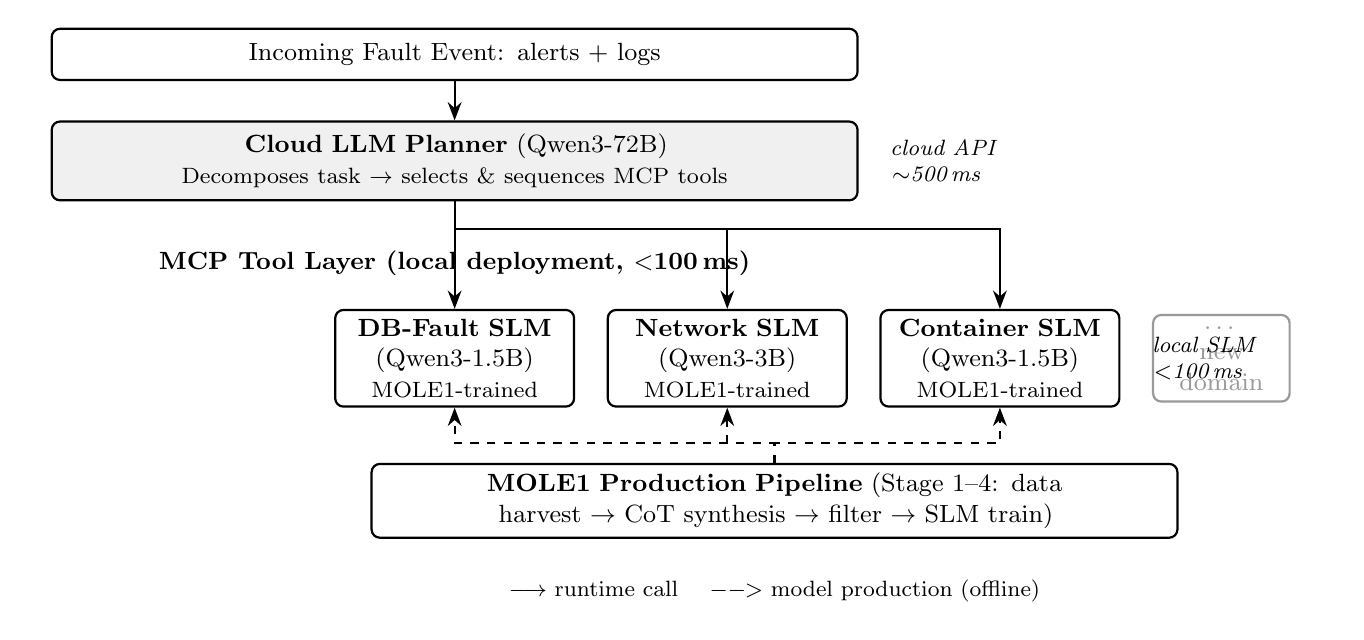
\begin{tikzpicture}[font=\small, node distance=0.5cm and 0.6cm]

% ── Layer 0: Fault event input ────────────────────────────────────────────────
\node[box=10cm, minimum height=0.65cm] (input)
  {Incoming Fault Event: alerts + logs};

% ── Layer 1: Cloud Planner ────────────────────────────────────────────────────
\node[greybox=10cm, minimum height=1.0cm, below=0.5cm of input] (planner)
  {\textbf{Cloud LLM Planner} (Qwen3-72B)\\
   \footnotesize Decomposes task $\to$ selects \& sequences MCP tools};

\node[left=0.05cm of planner, font=\footnotesize\itshape, rotate=90,
      anchor=south] {};

% ── Layer 2: MCP Tool endpoints ───────────────────────────────────────────────
\node[below=0.5cm of planner, font=\small\bfseries] (mcplabel)
  {MCP Tool Layer (local deployment, $<$100\,ms)};

\node[box=2.8cm, minimum height=1.1cm, below=0.3cm of mcplabel] (t1)
  {\textbf{DB-Fault SLM}\\(Qwen3-1.5B)\\{\footnotesize MOLE1-trained}};
\node[box=2.8cm, minimum height=1.1cm, right=0.4cm of t1] (t2)
  {\textbf{Network SLM}\\(Qwen3-3B)\\{\footnotesize MOLE1-trained}};
\node[box=2.8cm, minimum height=1.1cm, right=0.4cm of t2] (t3)
  {\textbf{Container SLM}\\(Qwen3-1.5B)\\{\footnotesize MOLE1-trained}};
\node[box=1.5cm, minimum height=1.1cm, right=0.4cm of t3,
      draw=black!40, text=black!40] (tdot)
  {\ldots\\new domain};

% ── Layer 3: MOLE1 production ────────────────────────────────────────────────
\node[box=10cm, minimum height=0.9cm,
      below=0.7cm of t2, xshift=0.6cm] (mole)
  {\textbf{MOLE1 Production Pipeline}
   (Stage 1–4: data harvest $\to$ CoT synthesis $\to$ filter $\to$ SLM train)};

% ── Arrows: input → planner ───────────────────────────────────────────────────
\draw[arrow] (input) -- (planner);

% ── Arrows: planner ↔ MCP tools ──────────────────────────────────────────────
\draw[arrow] (planner.south) -- ++(0,-0.35) -| (t1.north);
\draw[arrow] (planner.south) -- ++(0,-0.35) -| (t2.north);
\draw[arrow] (planner.south) -- ++(0,-0.35) -| (t3.north);

% ── Arrows: MOLE1 → MCP tools ────────────────────────────────────────────────
\draw[dasharrow] (mole.north) -- ++(0,0.25) -| (t1.south);
\draw[dasharrow] (mole.north) -- ++(0,0.25) -| (t2.south);
\draw[dasharrow] (mole.north) -- ++(0,0.25) -| (t3.south);

% ── Legend ────────────────────────────────────────────────────────────────────
\node[below=0.4cm of mole, align=left, font=\footnotesize] (leg) {%
  $\longrightarrow$ runtime call \quad
  $--\!\!>$ model production (offline)};

% ── Latency annotation ────────────────────────────────────────────────────────
\node[right=0.3cm of planner, align=left, font=\footnotesize\itshape,
      text width=2.5cm] {cloud API\\$\sim$500\,ms};
\node[right=0.3cm of t3, align=left, font=\footnotesize\itshape,
      text width=2.2cm] {local SLM\\$<$100\,ms};

\end{tikzpicture}

\caption{System architecture: cloud LLM as Planner orchestrates locally deployed
MCP-endpoint SLMs produced by the MOLE1 pipeline.}
\label{fig:arch}
\end{figure}

The cloud-hosted LLM (Qwen3-72B or equivalent) acts as a \textbf{Planner}: it
decomposes incoming fault events into sub-tasks, determines execution order, and
invokes the appropriate MCP tool endpoints.
Each MCP tool wraps an SLM that has been trained exclusively for one AIOps sub-scenario
(e.g., database slowdown diagnosis, network partition detection, container OOM triage).

The Planner–Executor split reflects the asymmetric nature of the two roles:
\begin{itemize}[itemsep=2pt]
  \item The Planner requires \emph{global semantic understanding} to decompose novel,
        multi-step fault events—a capability that demands the breadth of a large model.
  \item Each Executor requires \emph{deep, narrow expertise} in a single sub-domain—
        a capability that benefits from focused training on domain-specific CoT data,
        and which does \emph{not} benefit from the generalisation enforced by
        multi-task training on a large model.
\end{itemize}

This design also delivers the latency advantage: only the Planner call traverses the
cloud API ($\sim$500\,ms); all Executor SLM inferences run locally ($<$100\,ms), so
the end-to-end system responds in seconds even under high alert volume.

\subsubsection*{Why a Specialist SLM Can Outperform a General LLM}

The ``specialisation beats generalisation'' phenomenon is well-supported by the
distillation literature \citep{dss,ddk} and follows from two observations:
(i) a general LLM's parameters are shared across thousands of tasks, diluting
per-domain representational capacity \citep{slmsurvey}; (ii) an SLM fine-tuned
exclusively on domain-specific CoT data occupies a lower-dimensional subspace of
the parameter space that is tightly aligned with the target domain's inference
patterns, achieving higher precision despite far fewer parameters.
We will provide both empirical evidence (ablation studies varying model size and
training-data domain purity) and a capacity-allocation analysis to formalise this
intuition.

\textbf{Why not use the 7B medium model directly as executor?}
One may ask: since Qwen3-7B already possesses CoT capability and can run locally
on a single A10 GPU, why distil further to a 1.5B/3B model?
Three reasons: (1) \emph{accuracy}: a 1.5B SLM trained exclusively on
domain-verified CoT outperforms a 7B generalist on the target sub-task—the
domain-purity effect dominates the size effect at this scale \citep{ddk};
(2) \emph{deployment scale}: in a large platform with hundreds of hosts,
1.5B SLMs can be co-located with each service node at negligible memory overhead,
enabling zero-latency local inference without GPU scheduling;
(3) \emph{cost}: 1.5B inference costs $\approx$5$\times$ fewer FLOPs than 7B,
critical for high-frequency fault monitoring (thousands of events per minute).

\subsubsection*{Technical Advantages}

Comparing MOLE1 against existing LLM--SLM collaboration and SLM distillation methods:

\begin{enumerate}[leftmargin=*, itemsep=4pt]
  \item \textbf{Novelty.}
        Existing LLM--SLM collaboration frameworks (FrugalGPT, RouteLLM) assume
        specialist SLMs pre-exist and focus entirely on routing policy.
        Existing CoT distillation methods (STaR, Distilling Step-by-Step) require
        human-annotated CoT or a domain-aware teacher model.
        MOLE1 is the first to close the cold-start gap: automated specialist SLM
        production with \emph{no human annotation and no domain-aware teacher}, using
        only the ground-truth answer already present in historical records as verifier.
        This fills a critical blind spot in both lines of research.
  \item \textbf{Deployability.}
        The pipeline design is operationally transparent: collect historical records,
        run temperature-sampled CoT generation, filter by answer match, fine-tune with
        LoRA, and register as an MCP endpoint.
        Any Alibaba SRE team can apply the pipeline to a new AIOps sub-scenario within
        days, without ML expertise or labelling budget.
        The MCP-compliant packaging ensures plug-and-play integration with existing
        Planner infrastructure.
  \item \textbf{Effectiveness.}
        Domain-specific CoT training produces SLMs that match or exceed GPT-4-class
        LLMs on narrow tasks despite orders-of-magnitude fewer parameters—a
        well-established finding from the distillation literature \citep{dss,ddk} that
        MOLE1 extends to the cold-start, answer-verification regime.
        Empirical and theoretical analysis of the ``specialisation beats generalisation''
        phenomenon will be provided as part of the project output.
  \item \textbf{Efficiency.}
        MOLE1 adds zero labelling overhead and consumes a fraction of the compute
        required to train or query a general LLM.
        Inference-time savings are immediate: local SLM execution ($<$100\,ms)
        eliminates cloud API cost and latency for high-frequency AIOps monitoring tasks.
        The pipeline overhead is far smaller than the LLM API costs it replaces.
  \item \textbf{Generality.}
        MOLE1 requires only historical $\langle$input, output$\rangle$ pairs with
        automatically verifiable answers—a condition that holds across a wide range of
        industrial domains (customer-service triage, code-review classification,
        supply-chain anomaly detection).
        After the design is complete, it can be extended to multiple Alibaba business
        lines without domain-specific re-engineering, making it a broadly reusable
        cold-start asset well beyond the AIOps instantiation demonstrated here.
\end{enumerate}

% ══════════════════════════════════════════════════════════════════════════════
%  2. MILESTONE
% ══════════════════════════════════════════════════════════════════════════════
\section{Milestone}

\subsection{Duration of Project}
One year, commencing from the effective date of the Research Collaboration Agreement.

\subsection{Plan}

\begin{table}[H]
\centering
\caption{Project milestones and deliverables.}
\label{tab:milestone}
\renewcommand{\arraystretch}{1.4}
\begin{tabularx}{\linewidth}{c X X c}
\toprule
\textbf{Stage} & \textbf{Activities} & \textbf{Deliverable(s)} & \textbf{Period}\\
\midrule
M1 &
  \textbf{Pipeline Design \& Data Preparation.}
  Formalise MOLE1 algorithm; collect and pre-process AIOps
  $\langle$input, output$\rangle$ dataset; implement CoT candidate generation
  (Qwen3-7B) and answer-verification filter. &
  Dataset \& filter module; technical report. &
  Month 1–3 \\
\midrule
M2 &
  \textbf{SLM Training \& Benchmarking.}
  Fine-tune SLMs on verified CoT triples; conduct comparison experiments
  against general LLM baselines on AIOps benchmarks;
  specialisation-mechanism analysis. &
  Trained SLM models; experiment report;
  draft of CCF-A paper \#1. &
  Month 4–7 \\
\midrule
M3 &
  \textbf{MCP Packaging \& System Integration.}
  Wrap each SLM as an MCP tool endpoint; integrate Planner (Qwen3-72B)
  with MCP tool layer; end-to-end latency and accuracy evaluation. &
  Open-source MCP toolkit; system demo;
  draft of CCF-A paper \#2. &
  Month 8–9 \\
\midrule
M4 &
  \textbf{Evaluation, Patent Filing \& Final Deliverables.}
  Full system evaluation; user study with Alibaba stakeholders;
  patent applications; final project report. &
  Final report; published/submitted papers;
  patent applications (1–2). &
  Month 10–12 \\
\bottomrule
\end{tabularx}
\end{table}

\begin{figure}[H]
\centering
% 图4：项目甘特图（简洁版，纯 TikZ）
\begin{tikzpicture}[font=\small, x=0.80cm, y=0.68cm]

\def\nmonths{12}
\def\nrows{4}

% ── 月份表头 ───────────────────────────────────────────────────────────────────
\foreach \m in {1,...,12}{
  \draw[gray!30] (\m,0) -- (\m,-\nrows-0.1);
  \node[above, font=\footnotesize] at (\m-0.5,0) {\m};
}
\draw[gray!30] (0,0) -- (0,-\nrows-0.1);
\draw[thick] (0,0) -- (12,0);
\node[above, font=\footnotesize\bfseries] at (6,0.38) {月份};

% ── 行标签（右对齐，统一格式） ────────────────────────────────────────────────
\node[left=0.15cm, align=right, font=\footnotesize, text width=3.2cm] at (0,-0.5)
  {\textbf{M1：}流水线与数据};
\node[left=0.15cm, align=right, font=\footnotesize, text width=3.2cm] at (0,-1.5)
  {\textbf{M2：}SLM 训练};
\node[left=0.15cm, align=right, font=\footnotesize, text width=3.2cm] at (0,-2.5)
  {\textbf{M3：}系统集成};
\node[left=0.15cm, align=right, font=\footnotesize, text width=3.2cm] at (0,-3.5)
  {\textbf{M4：}最终交付};

% ── 甘特条 ────────────────────────────────────────────────────────────────────
% M1：第 1–3 月
\fill[black!15, draw=black!60, thick] (0,-0.15) rectangle (3,-0.85);
\node[font=\footnotesize] at (1.5,-0.5) {数据采集与过滤};

% M2a：第 1–7 月（CoT 生成 + SLM 训练）
\fill[black!22, draw=black!60, thick] (1,-1.15) rectangle (7,-1.85);
\node[font=\footnotesize] at (3.5,-1.5) {CoT 合成 + SFT/GRPO 训练};

% M2b：第 7–10 月（跨域验证，探索性）
\fill[black!8, draw=black!50, thick, dashed] (7,-1.15) rectangle (10,-1.85);
\node[font=\scriptsize, align=center] at (8.5,-1.5) {跨域验证\\（探索性）};

% M3：第 6–9 月
\fill[black!15, draw=black!60, thick] (6,-2.15) rectangle (9,-2.85);
\node[font=\footnotesize] at (7.5,-2.5) {MCP 集成与评估};

% M4：第 9–12 月
\fill[black!22, draw=black!60, thick] (9,-3.15) rectangle (12,-3.85);
\node[font=\footnotesize] at (10.5,-3.5) {验收与交付};

% ── 里程碑菱形标记 ────────────────────────────────────────────────────────────
\node[diamond, draw=black, fill=black, inner sep=2.0pt] at (3,-0.5) {};
\node[diamond, draw=black, fill=black, inner sep=2.0pt] at (7,-1.5) {};
\node[diamond, draw=black, fill=black, inner sep=2.0pt] at (9,-2.5) {};
\node[diamond, draw=black, fill=black, inner sep=2.0pt] at (12,-3.5) {};

% 里程碑标签（上方）
\node[above=0.06cm, font=\scriptsize\bfseries] at (3,-0.15)  {M1};
\node[above=0.06cm, font=\scriptsize\bfseries] at (7,-1.15)  {M2};
\node[above=0.06cm, font=\scriptsize\bfseries] at (9,-2.15)  {M3};
\node[above=0.06cm, font=\scriptsize\bfseries] at (12,-3.15) {M4};

% ── 外框 ─────────────────────────────────────────────────────────────────────
\draw[thick] (0,0) rectangle (12,-\nrows-0.1);

\end{tikzpicture}

\caption{Project Gantt chart across four milestones.}
\label{fig:gantt}
\end{figure}

% ══════════════════════════════════════════════════════════════════════════════
%  3. DELIVERABLES
% ══════════════════════════════════════════════════════════════════════════════
\section{Deliverable(s)}

The following final deliverables are committed for this project.

\begin{enumerate}[leftmargin=*, itemsep=4pt]
  \item \textbf{Algorithm prototype system.}
        Complete MOLE1 cold-start SLM production pipeline: data harvesting module,
        CoT candidate generation, answer-verification filter, SLM fine-tuning (SFT +
        LoRA), and MCP endpoint packaging. Source code released open-source on GitHub;
        fully reproducible experimental environment provided.
  \item \textbf{MCP-compliant AIOps tool-endpoint toolkit.}
        Packaged SLM executors for 3+ AIOps sub-scenarios (database-layer faults,
        network partition events, container resource exhaustion), with documentation
        and integration guide for the Planner layer.
  \item \textbf{Design documents.}
        Submit 1 overview design document (system architecture and pipeline specification)
        and 1 detailed design document (algorithm, evaluation protocol, and
        deployment guide).
  \item \textbf{Paper targets.}
        Publish 2 papers at CCF-A or equivalent top venues (e.g., NeurIPS, ICML, ACL,
        ICSE, FSE), covering MOLE1 methodology and AIOps evaluation results.
  \item \textbf{Patent targets.}
        Submit 1--2 invention patent applications on cold-start CoT synthesis and
        MCP endpoint packaging (China or international).
  \item \textbf{Technical targets.}
        Compared with existing AIOps approaches: SLMs produced by MOLE1 achieve
        remediation-action accuracy within 5\% of GPT-4-class LLMs, reduce
        per-inference latency by $>$10$\times$ (from $\sim$1\,s to $<$100\,ms),
        and reduce per-query token cost to zero (local inference).
  \item \textbf{Business targets.}
        System deployed and launched in 3+ Alibaba AIOps business scenarios, with
        documented performance improvement relative to LLM-only baseline.
  \item \textbf{Project acceptance report.}
        Submit 1 final acceptance test report at project conclusion.
  \item \textbf{Student co-training and internship.}
        Jointly train 2--3 graduate students participating in this project; provide
        Alibaba SRE team internship opportunities during the project period
        (indicative: Months 4--9, subject to Alibaba schedule).
\end{enumerate}

\begin{table}[H]
\centering
\caption{Summary of deliverables and delivery mode.}
\renewcommand{\arraystretch}{1.4}
\begin{tabularx}{\linewidth}{X l p{4.8cm}}
\toprule
\textbf{Description} & \textbf{Mode of Delivery} & \textbf{Remarks}\\
\midrule
Prototype system: MOLE1 cold-start SLM production pipeline &
  Source code (open-source) &
  Reproducible; released on GitHub \\
MCP-compliant AIOps tool-endpoint toolkit &
  Source code + documentation &
  Compatible with standard MCP protocol \\
Overview and detailed design documents &
  Technical reports &
  Submitted at M1 and M3 milestones \\
2 academic papers on MOLE1 methodology and AIOps evaluation &
  Academic papers &
  Targeting CCF-A or equivalent top venues \\
1--2 invention patents on cold-start CoT synthesis and MCP packaging &
  Patent applications &
  China or international patents \\
Interim and final project reports &
  Project reports &
  Submitted per agreed schedule \\
Graduate student internship at Alibaba &
  Personnel arrangement &
  2--3 PhD students; Months 4--9 (indicative) \\
\bottomrule
\end{tabularx}
\end{table}

% ══════════════════════════════════════════════════════════════════════════════
%  4. HUMAN RESOURCES, EQUIPMENT AND BUDGET
% ══════════════════════════════════════════════════════════════════════════════
\section{Human Resources, Equipment and Budgetary Plan}

\subsection{Personnel}

\begin{table}[H]
\centering
\renewcommand{\arraystretch}{1.4}
\small
\begin{tabular}{p{2.4cm} p{3.2cm} r r r p{1.6cm} p{1.6cm}}
\toprule
\textbf{Name} & \textbf{Profile} & \textbf{RMB/mo.} & \textbf{Period} &
\textbf{Total} & \textbf{Role} & \textbf{Internship}\\
\midrule
\textit{<FILL: PI>} &
  \textit{<FILL: Prof.>},\newline \textit{<FILL: Univ.>} &
  12{,}000 & 3\,mo. & 36{,}000 & PI & ---\\
\textit{<FILL: PhD 1>} &
  PhD Student,\newline \textit{<FILL: Univ.>} &
  12{,}000 & 12\,mo. & 144{,}000 & Research Asst. & Mo. 4--6\\
\textit{<FILL: PhD 2>} &
  PhD Student,\newline \textit{<FILL: Univ.>} &
  12{,}000 & 12\,mo. & 144{,}000 & Research Asst. & Mo. 7--9\\
\midrule
\multicolumn{4}{r}{\textbf{Sub-total Personnel (a)}} & \multicolumn{3}{r}{\textbf{RMB 324{,}000}}\\
\bottomrule
\end{tabular}
\end{table}

\noindent\small\textit{Internship periods are indicative; exact dates subject to Alibaba SRE team schedule.}

\subsection{Equipment \& Supplies}

\begin{table}[H]
\centering
\renewcommand{\arraystretch}{1.4}
\begin{tabularx}{\linewidth}{X r r p{5cm}}
\toprule
\textbf{Item} & \textbf{Unit Price (RMB)} & \textbf{Total (RMB)} & \textbf{Remarks}\\
\midrule
GPU cloud computing (A100 node-hours) & — & 91,000 &
  For SLM training runs (Stage 2--3)\\
Local inference server (lease/purchase) & 50,000 & 50,000 &
  MCP endpoint deployment \& latency testing\\
Conference travel (2 venues) & 15,000 & 30,000 &
  Domestic + international top-venue presentation\\
Open-access publication fees & 10,000 & 20,000 &
  ACL Anthology / NeurIPS open access\\
\midrule
\multicolumn{2}{r}{\textbf{Sub-total Research Expenses (b)}} & \textbf{191,000} & \\
\bottomrule
\end{tabularx}
\end{table}

\subsection{Budgetary Plan}

\begin{table}[H]
\centering
\renewcommand{\arraystretch}{1.5}
\begin{tabularx}{\linewidth}{l X r}
\toprule
\textbf{Item} & \textbf{Remarks} & \textbf{Amount (RMB)}\\
\midrule
(a) Total Personnel Expenses & See Section 4.1 & 324,000\\
(b) Total Research Expenses  & See Section 4.2 & 191,000\\
(c) Indirect Cost            &
  University overhead: $16.5\%\times(\text{a}+\text{b})
  = 16.5\%\times 515{,}000 \approx 85{,}000$ & 85,000\\
\midrule
\textbf{Grand Total} & (a) + (b) + (c) & \textbf{600,000}\\
\bottomrule
\end{tabularx}
\end{table}

% ══════════════════════════════════════════════════════════════════════════════
%  5. BIOGRAPHICAL SKETCHES OF PRINCIPAL INVESTIGATOR(S)
% ══════════════════════════════════════════════════════════════════════════════
\section{Biographical Sketches of Principal Investigator(s)}

\textbf{\textit{<FILL: PI Full Name>}}\\
\textit{<FILL: Professor / Associate Professor / Tenure-track Assistant Professor>},
\textit{<FILL: Department / School Name>},
\textit{<FILL: University Full Name>}\\
Email: \textit{<FILL: pi@university.edu>} \quad
Homepage: \textit{<FILL: https://pi-homepage-url>}

\textbf{Education:}
\begin{itemize}[leftmargin=*, itemsep=1pt]
  \item PhD, \textit{<FILL: Dept., University>}
        (Advisor: Prof.\ \textit{<FILL: Advisor Name>})
  \item MS/BEng, \textit{<FILL: Dept., University>}
\end{itemize}

\textbf{Research Interests:}
Large Language Models, Knowledge Distillation, AIOps and Intelligent Operations,
Automated Machine Learning, Intelligent Software Systems.

\textbf{Representative Publications (recent 5 years):}
\begin{enumerate}[leftmargin=*, itemsep=2pt]
  \item \textit{<FILL: Author(s). ``Title.'' Venue (CCF-A / top venue), Year.
        [Note role: first author / corresponding author]>}
  \item \textit{<FILL: Author(s). ``Title.'' Venue (CCF-A / top venue), Year.>}
  \item \textit{<FILL: Author(s). ``Title.'' Venue (CCF-A / top venue), Year.>}
  \item \textit{<FILL: Author(s). ``Title.'' Venue (CCF-A / top venue), Year.>}
  \item \textit{<FILL: Author(s). ``Title.'' Venue (CCF-A / top venue), Year.>}
\end{enumerate}

\textbf{Selected Grants and Awards:}
\begin{itemize}[leftmargin=*, itemsep=2pt]
  \item \textit{<FILL: Funding body, Project title, Total amount (RMB/USD), Role (PI/Co-PI), Year(s)>}
  \item \textit{<FILL: Funding body, Project title, Total amount, Role, Year(s)>}
  \item \textit{<FILL: Award name, Awarding body, Year>}
\end{itemize}

\textbf{Academic Service:}
\begin{itemize}[leftmargin=*, itemsep=1pt]
  \item (Senior) PC Member / Reviewer:
        \textit{<FILL: list top venues, e.g., NeurIPS, ICML, ACL, ICSE, FSE, KDD>}
  \item \textit{<FILL: Tutorial speaker / Workshop organiser at top venue, Year>}
\end{itemize}

\medskip
\noindent\textbf{Note: Specific Relevant Experience for This Proposal.}

\begin{enumerate}[leftmargin=*, itemsep=3pt]
  \item \textit{<FILL: ``Published N papers directly in this direction at [list CCF-A venues with years], of which N are as first or corresponding author.
        Representative papers: [1] \ldots\ [2] \ldots''>}
  \item \textit{<FILL: ``During [company] research collaboration / internship ([duration]),
        was main member of [project name], an [LLM distillation / AIOps / AutoML]-based
        system.  Led deployment of [specific model/component] across [N] business lines
        ([list product names]), achieving [concrete quantified result, e.g., ``50\% latency
        reduction'' or ``X\% accuracy improvement on fault diagnosis''].''>}
  \item \textit{<FILL: ``Gave [tutorial / invited talk] on [relevant topic, e.g.,
        ``LLM--SLM collaboration'' or ``automated AIOps''] at CCF-A conference(s)
        [list venues and years], receiving [wide attention / positive reviews].
        Authored survey paper [title, arXiv/venue, year] on the topic.''>}
\end{enumerate}

% ══════════════════════════════════════════════════════════════════════════════
%  6. REFERENCES
% ══════════════════════════════════════════════════════════════════════════════
\section{References}

\bibliographystyle{abbrvnat}
\bibliography{refs}

\end{document}
